\newpage
\chapter{Simulation and Performance Estimation}
Before finalizing the manufacturing files, critical subsystems of the hardware design were simulated to validate mathematical sizing, verify layout choices and ensure compliance with the system's requirements.

\section{RF Antenna Design and Matching Network Tuning}
To guarantee reliable Bluetooth communication, the physical PCB layout of the antenna and its associated feedline was imported into Keysight Advanced Design System (ADS) and analyzed using the RFPro 3D electromagnetic (EM) simulation tool. This step was necessary because the performance results reported in the IFA antenna application report \cite{rf_ifa_ar} were obtained using a substrate thickness of \SI{1}{\milli\meter}, whereas the final design employs a different PCB stack-up. Since antenna characteristics are strongly influenced by substrate properties, including thickness and dielectric constant, a dedicated EM simulation was performed to accurately characterize the implemented RF structure, as shown in Figure~\ref{fig:ads_em_simulation}.

The simulation was used to extract the S-parameters of the RF section, with particular focus on the input reflection coefficient ($S_{11}$) and voltage standing wave ratio ($VSWR$), in order to evaluate the impedance matching between the MCU RF pin and the antenna. Based on the simulation results, the matching network component values were validated to closely match the nominal \SI{50}{\ohm} system impedance, thereby minimizing reflected power and maximizing power transfer to the antenna.

As shown in Figure~\ref{fig:s11_simulation}, the optimized design achieved an $S_{11}$ below \SI{-20}{\deci\bel} at the center frequency of \SI{2.45}{\giga\hertz}, corresponding to a very low reflected power level. Furthermore, the VSWR, reported in Figure~\ref{fig:vswr_simulation}, remained below 2 over an approximate bandwidth of \SI{200}{\mega\hertz}, fully covering the \SI{2.4}{\giga\hertz} ISM band and providing adequate tolerance against manufacturing variations and environmental detuning effects.

\begin{figure}[H]
    \centering
    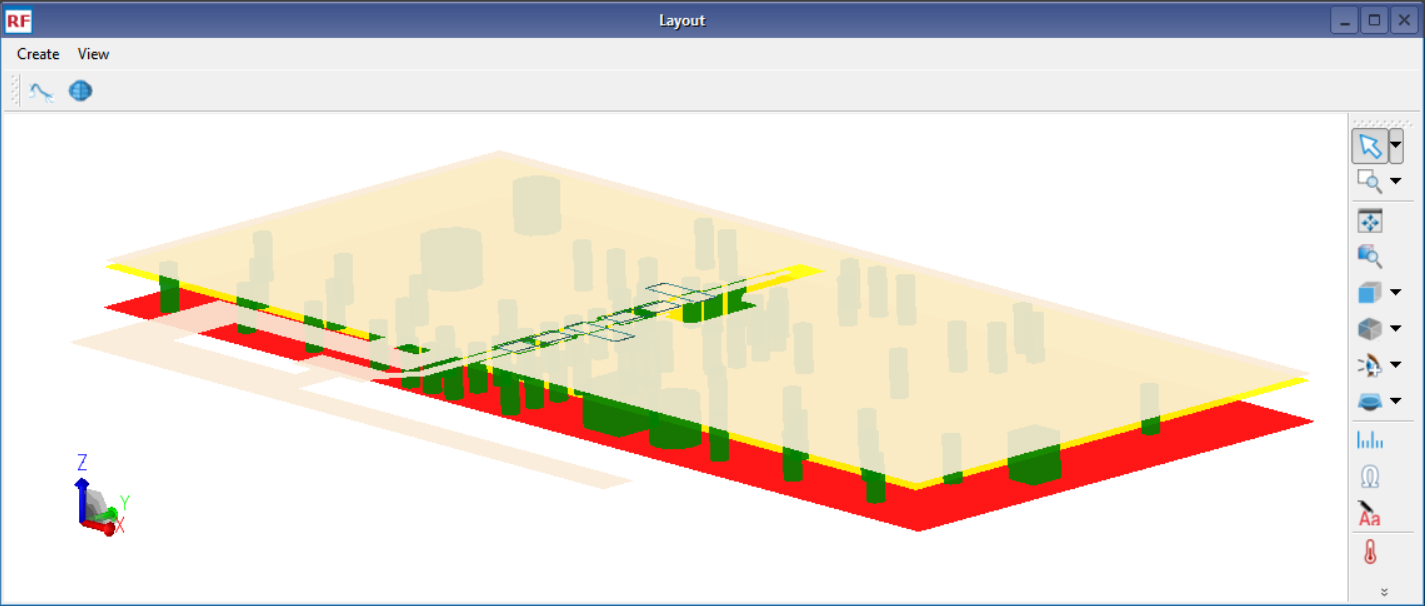
\includegraphics[width=0.9\linewidth]{figures/2_HW_figures/ads_em_simulation.png}
    \caption{3D EM simulation setup of the antenna and feedline in ADS RFPro.}
    \label{fig:ads_em_simulation}
\end{figure}

\begin{figure}[H]
    \centering
    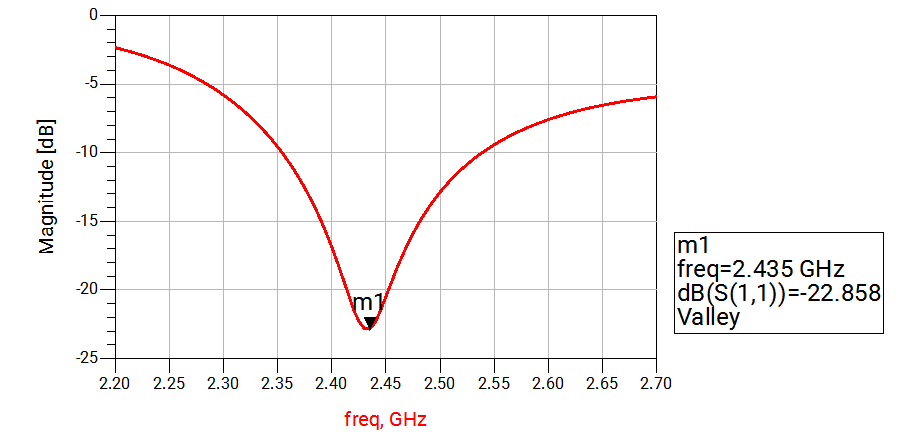
\includegraphics[width=0.85\linewidth]{figures/2_HW_figures/s11.png}
    \caption{Simulated $S_{11}$ (return loss) of the antenna and matching network obtained from simulation.}
    \label{fig:s11_simulation}
\end{figure}

\begin{figure}[H]
    \centering
    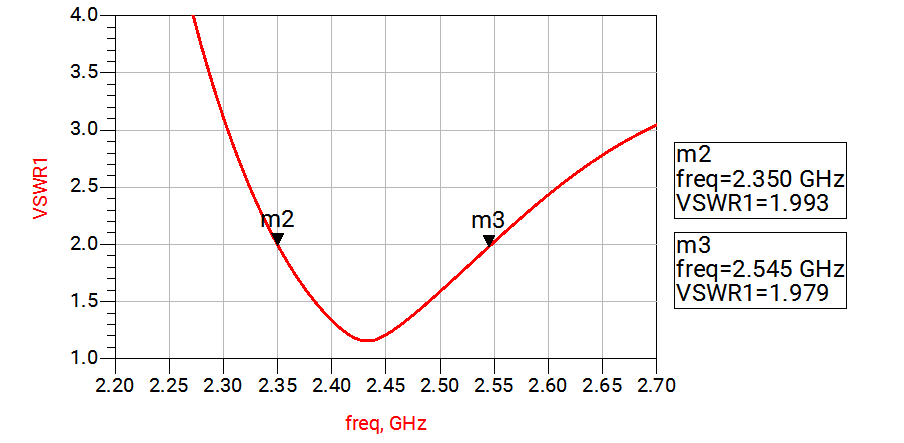
\includegraphics[width=0.85\linewidth]{figures/2_HW_figures/vswr.png}
    \caption{Simulated VSWR of the antenna and matching network showing impedance matching performance around 2.45 GHz.}
    \label{fig:vswr_simulation}
\end{figure}

\section{NTC Circuit with High-Side Enable Switch}
Temperature monitoring is performed using an NTC thermistor configured in a voltage divider. To satisfy the strict OFF-state power consumption requirement, this divider is not continuously powered. Instead, as explained in section~\ref{ntc}, it is driven by a high-side enable switch controlled by a microcontroller GPIO, ensuring current only flows during active ADC sampling.

A SPICE transient simulation was performed to analyze the dynamic response of this switching circuit (see Figure~\ref{fig:ntc_ltspice}). The simulation verified the turn-on settling time. Because the NTC node contains parasitic and filtering capacitance, the simulation determined the exact delay required between asserting the enable signal and triggering the ADC conversion. This ensures the analog voltage is sampled only after it has fully stabilized, guaranteeing temperature measurement accuracy without wasting power.

Based on the simulation results, the RC time constant of the sensing network was tuned to achieve a trade-off between settling time and noise filtering. In particular, the capacitance value of \SI{100}{\nano\farad} was selected to achieve attenuation higher than \SI{60}{\decibel} at the \SI{1.7}{\mega\hertz} dc-dc switching frequency, while still meeting the required acquisition timing defined by the system sampling constraints. In parallel, the gate pull-up resistor value of \SI{100}{\kilo\ohm} was chosen to ensure a fast enough turn-off of the sensing branch, preventing residual conduction during low-power operation while avoiding unnecessary quiescent current consumption.

The dynamic response analysis of the circuit allows the extraction of the settling time after the enable signal is asserted (see Figure~\ref{fig:ntc_spice_transient}). The measured rise time is approximately \SI{3}{\milli\second}, which defines the minimum safe acquisition window for the ADC conversion. This ensures that the sampled voltage is fully stabilized and free from transient effects. Based on this result, ON-time of \SI{5}{\milli\second} is chosen as a safety margin over the simulated settling time to guarantee robust operation under worst-case conditions.

\begin{figure}[H]
    \centering
    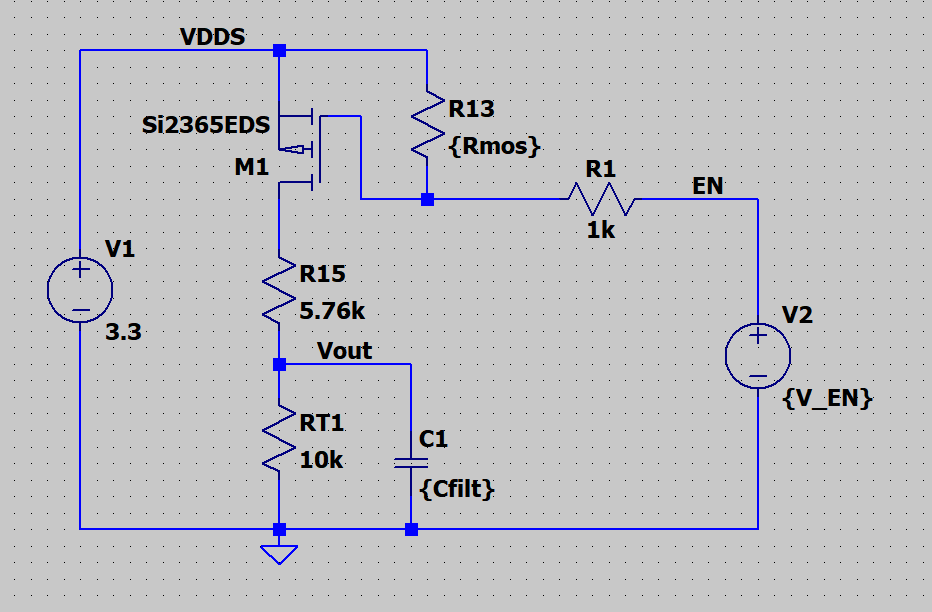
\includegraphics[width=0.75\textwidth]{figures/2_HW_figures/ntc_ltspice.png}
    \caption{LTspice simulation setup of the NTC sensing circuit used for transient and steady-state response analysis.}
    \label{fig:ntc_ltspice}
\end{figure}

\begin{figure}[H]
    \centering
    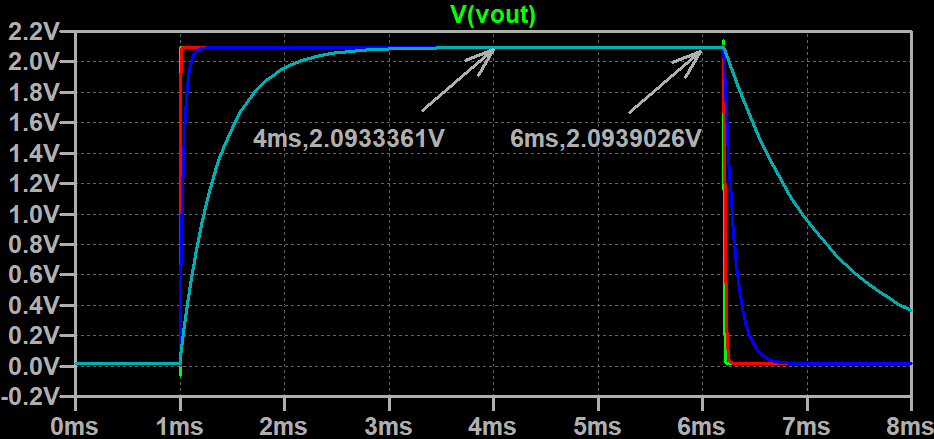
\includegraphics[width=0.75\textwidth]{figures/2_HW_figures/ntc_spice_transient.png}
    \caption{SPICE transient simulation of the NTC sensing circuit showing turn-on settling behavior.}
    \label{fig:ntc_spice_transient}
\end{figure}

After validation of the chosen component values in terms of dynamic response, an estimation of the power consumption was performed to quantify the benefit of the enable-controlled sensing circuit. The analysis compares the average power dissipation in both the always-on configuration and the duty-cycled implementation enabled by the MOSFET control stage.

The results show that, during a \SI{200}{\milli\second} period, the sensing network with the enable circuit dissipates an average power of \SI{5.55}{\micro\watt}, while in the always-enabled configuration the average power consumption increases to \SI{138}{\micro\watt}. This corresponds to an energy saving of around \SI{96}{\percent} over the defined duty cycle, significantly improving OFF-state battery life and supporting the system requirement defined in Requirement~\ref{req:pwr_battery}.



\section{System Power Consumption Evaluation}
\label{sec:system_power_consumption}

After the device selection and the definition of the main firmware timing parameters, the power consumption of WattMate can be estimated. 
This evaluation is used to verify the requirements related to the power consumption of the system regarding the ON-state efficiency and the idle battery life.

\subsection{Power Estimation Methodology}
\label{sec:power_estimation_methodology}

The total power dissipated by WattMate is evaluated by separating the losses introduced by the internal electronics from the power dissipated directly in the measured USB power path. 
For any given operating condition, the total dissipated power is modeled as:
\begin{equation}
	P_{WattMate} = P_{electronics} + P_{shunt} = (P_{components} + P_{DC/DC}) + P_{shunt}
\end{equation}

where \(P_{electronics}\) is the power required to supply the internal electronics of WattMate, while \(P_{shunt}\) is the power dissipated on the shunt resistor used to sense the USB bus current.

\(P_{electronics}\) can be further divided into the average power required by the internal circuitry and the average losses introduced by the power supply stage. 

\paragraph{Shunt dissipation.}
The shunt resistor is placed directly in the measured USB power path. 
Its power dissipation therefore depends on the current flowing through the monitored bus:
\begin{equation}
	P_{shunt} = I_{bus}^{2} \cdot R_{shunt}
\end{equation}

\paragraph{Component average power.}
The average consumption of each relevant electronic subsystem is estimated by assigning an active current, a sleep current, and a duty cycle. 
For each block, the average current is then computed as:
\begin{equation}
	\label{current_avg_formula}
	I_{avg} = D \cdot I_{ON} + \left(1-D\right) \cdot I_{sleep}
\end{equation}

where \(D\) is the fraction of time during which the block is ON in the considered operating condition.

The total average current required by the internal electronics is then obtained by summing the contribution of all powered blocks:
\begin{equation}
	I_{components} = \sum_k I_{avg,k}
\end{equation}

Assuming a regulated internal supply voltage \(V_{DD}\), the average power delivered to the components is:
\begin{equation}
	P_{components} = V_{DD} \cdot I_{components}
\end{equation}

The ON and sleep current values are defined once and then reused in the ON-state and idle evaluations. 
The duty cycles, instead, depend on the considered operating condition and are therefore evaluated separately for each scenario.

\paragraph{DC/DC converter losses.}
The DC/DC converter contribution is modeled as the sum of its quiescent power and conversion losses:
\begin{equation}
	P_{DC/DC} = P_{quiescent} + P_{loss}
\end{equation}

The quiescent term represents the power required by the converter control circuitry, while \(P_{loss}\) accounts for the finite conversion efficiency. 
Since the converter efficiency depends on the output current, \(P_{loss}\) is not estimated using only a single average current value. 
Instead, the detailed estimation is performed by defining a current profile and evaluating the converter efficiency in different current regions, as described in Section~\ref{sec:dcdc_loss_estimation}.

\subsection{Power Supply Loss Estimation}
\label{sec:dcdc_loss_estimation}

The DC/DC converter loss cannot be estimated accurately using only a single average output current, because the converter efficiency strongly depends on its output current. 
This effect is especially relevant at low load, where the efficiency of a switching converter can decrease significantly compared to its nominal value. 
For this reason, the duty cycles \(D\), defined for each electronic subsystem in each operating condition under evaluation, are used to define a current profile.

The current profile is built using a simple rule: each subsystem is considered ON at the start of the cycle and remains ON for a percentage of the cycle determined by its duty-cycle value. 
This current profile is still an approximation, because the complete dynamic behaviour of the device can only be verified experimentally, but it provides a more realistic design-stage estimate than assuming a constant output current.

This current profile is then used to evaluate the conversion loss by dividing it into representative output-current regions. 
For each region, the corresponding efficiency is extracted from the DC/DC converter datasheet. 
If \(P_{out,i}\), \(\eta_i\), and \(\alpha_i\) are respectively the output power, efficiency, and time fraction of region \(i\), the average conversion loss is computed as:
\begin{equation}
	P_{loss} = \sum_i \alpha_i \cdot P_{out,i} \cdot \left(\frac{1}{\eta_i} - 1\right)
\end{equation}

The quiescent power is evaluated under the worst-case input voltage:
\begin{equation}
	P_{quiescent} = V_{worst} \cdot I_{quiescent}
\end{equation}

The total DC/DC contribution is then:
\begin{equation}
	P_{DC/DC} = P_{quiescent} + P_{loss}
\end{equation}



\subsection{ON-state and Idle Currents for Subsystems}
\label{sec:on_idle_currents_subsystems}

After defining the duty cycle of each subsystem, the corresponding ON and idle currents must be assigned. 
These values are used to compute the average current contribution of each block according to the methodology introduced in Section~\ref{sec:power_estimation_methodology}.

When possible, the currents are taken directly from the component datasheets.

\paragraph{MCU core.}
The CC2640R2F datasheet models the ON MCU current as a fixed base contribution plus a frequency-dependent term~\cite{mcu_datasheet}. 
Since the firmware runs with a \(48\,\mathrm{MHz}\) system clock, the ON current used for the MCU core is:
\begin{equation}
	I_{MCU,ON} = I_{base} + I_{freq} \cdot f_{CPU}
	= 1.45\,\mathrm{mA} + 0.031\,\mathrm{mA/MHz} \cdot 48\,\mathrm{MHz}
	= 2.94\,\mathrm{mA}
\end{equation}

When the core is not ON, the standby current with retention is used as idle-state contribution~\cite{mcu_datasheet}:
\begin{equation}
	I_{MCU,idle} \simeq 1.1\,\mu\mathrm{A} = 0.0011\,\mathrm{mA}
\end{equation}

\paragraph{I\textsuperscript{2}C peripheral and pull-up resistors.}
The I\textsuperscript{2}C bus contribution is composed of two terms: the internal I\textsuperscript{2}C peripheral current of the MCU and the current dissipated by the external pull-up resistors on SDA and SCL.

The I\textsuperscript{2}C peripheral current is taken from the CC2640R2F datasheet~\cite{mcu_datasheet}:
\begin{equation}
	I_{I2C,periph,ON} = 12\,\mu\mathrm{A} = 0.012\,\mathrm{mA}
\end{equation}

The external pull-up resistors have a value of \(10\,\mathrm{k\Omega}\). 
When one I\textsuperscript{2}C line is driven low, the corresponding pull-up current is:
\begin{equation}
	I_{PU,line} = \frac{V_{DD}}{R_{PU}} = \frac{3.3\,\mathrm{V}}{10\,\mathrm{k\Omega}} = 0.33\,\mathrm{mA}
\end{equation}

During an active I\textsuperscript{2}C transfer, SCL is low for approximately half of the clock period, while the SDA level depends on the transmitted data. 
For a simple average estimate, the two bus lines are modeled as one equivalent pull-up resistor conducting during I\textsuperscript{2}C activity. 
The total ON current associated with the I\textsuperscript{2}C block is therefore:
\begin{equation}
	I_{I2C,ON} = I_{I2C,periph,ON} + I_{PU,I2C,ON}
	= 0.012\,\mathrm{mA} + 0.33\,\mathrm{mA}
	= 0.342\,\mathrm{mA}
\end{equation}

When the bus is inactive, both lines are pulled high and no static current flows through the pull-up resistors. 
The I\textsuperscript{2}C block is therefore considered idle outside the bus activity windows.

\paragraph{Other MCU peripheral contributions.}
Other MCU-side peripherals are grouped together. 
In the considered firmware configuration, this contribution includes two timers and the RF core idle contribution~\cite{mcu_datasheet}:
\begin{equation}
	I_{periph,ON} = 2 \cdot I_{timer} + I_{RFcore,idle}
	= 2 \cdot 113\,\mu\mathrm{A} + 237\,\mu\mathrm{A}
	= 463\,\mu\mathrm{A}
	= 0.463\,\mathrm{mA}
\end{equation}

This RF-core value represents the idle RF-core contribution and is kept separate from the BLE TX and RX radio currents, which are modeled independently.



\paragraph{External subsystems.}
The PAC1951 measurement sensor is set to the Normal Sampling Profile, defined in Section~\ref{PAC_Application_Task}, during ON-state measurement operation. 
In this configuration, the sensor samples one input channel at \(64\,\mathrm{SPS}\). 
During idle-state operation, the PAC1951 is set to the Idle Sampling Profile, also defined in Section~\ref{PAC_Application_Task}, where one input channel is sampled at \(8\,\mathrm{SPS}\). 
Given these operating conditions, the ON-state and idle-state currents of the PAC1951 are taken from the component datasheet~\cite{pac1951_datasheet}.

The NTC branch is powered only during temperature acquisition. 
Its ON current is computed from the circuit shown in Figure~\ref{fig:ntc_circuit}, using the thermistor value at \(25\,^\circ\mathrm{C}\), resulting in \(0.20\,\mathrm{mA}\)~\cite{ntc_datasheet}. 
When the NTC control MOSFET is disabled, the NTC branch is considered idle, and its current consumption is assumed to be zero.

The OLED display current is taken from the display datasheet for the reference condition of approximately \(50\%\) pixels ON~\cite{oled_datasheet}. 
When the display is disabled, its contribution is considered zero.

\paragraph{BLE radio currents.}
The BLE TX and RX currents are taken from the CC2640R2F datasheet~\cite{mcu_datasheet}. 
For the TX case, the \(+5\,\mathrm{dBm}\) value is used as a conservative estimate:
\begin{equation}
	I_{BLE,TX,ON} = 9.10\,\mathrm{mA}
\end{equation}

For RX activity, the ON-mode RX current is used:
\begin{equation}
	I_{BLE,RX,ON} = 6.10\,\mathrm{mA}
\end{equation}

The radio is considered idle outside the TX and RX activity windows estimated in Section~\ref{sec:standard_use_cycle}.

\begin{table}[H]
	\centering
	\small
	\caption{ON and idle current values used for the subsystem power estimate.}
	\label{tab:on_idle_currents_subsystems}
	\begin{tabular}{p{0.24\textwidth} p{0.18\textwidth} p{0.18\textwidth}}
		\toprule
		\textbf{Subsystem} & \textbf{\(I_{ON}\)} & \textbf{\(I_{idle}\)} \\
		\midrule
		MCU core &
		\(2.94\,\mathrm{mA}\) &
		\(0.0011\,\mathrm{mA}\) \\
		
		I\textsuperscript{2}C block &
		\(0.342\,\mathrm{mA}\) &
		\(0\,\mathrm{mA}\) \\
		
		Other MCU peripherals &
		\(0.463\,\mathrm{mA}\) &
		\(0\,\mathrm{mA}\) \\
		
		PAC1951 sensor &
		\(0.010\,\mathrm{mA}\) &
		\(0.005\,\mathrm{mA}\) \\
		
		NTC branch &
		\(0.200\,\mathrm{mA}\) &
		\(0\,\mathrm{mA}\) \\
		
		OLED display &
		\(32\,\mathrm{mA}\) &
		\(0\,\mathrm{mA}\) \\
		
		BLE TX &
		\(9.10\,\mathrm{mA}\) &
		\(0\,\mathrm{mA}\) \\
		
		BLE RX &
		\(6.10\,\mathrm{mA}\) &
		\(0\,\mathrm{mA}\) \\
		\bottomrule
	\end{tabular}
\end{table}













\subsection{ON-State Operating Efficiency}
\label{sec:operating_efficiency}

In this section, the power consumption of WattMate is evaluated under ON-state operating conditions, namely when non-negligible power is flowing through the USB power bus and WattMate is actively measuring the electrical state of the same bus.

The efficiency is evaluated under the worst-case bus operating point considered for the design:

\begin{equation}
	\label{eq:on_state_worst_case_conditions}
	V_{worst} = 21\,\mathrm{V}
	\qquad
	I_{worst} = 5\,\mathrm{A}
\end{equation}

These values represent the maximum voltage and current used to verify the ON-state efficiency requirement. 
They are used to compute the worst-case shunt dissipation, the worst-case monitored bus power, and the DC/DC quiescent contribution under maximum input voltage.

 

\paragraph{Standard Use Cycle}
\label{sec:standard_use_cycle}

The power consumption of WattMate in ON-state depends on the way the user interacts with the device. 
This is especially true for features related to the human interface, such as the OLED display and the BLE connection with the mobile application. 
For this reason, a standard use cycle is defined to estimate the average consumption in a repeatable way.

The standard use cycle is defined over \(1\,\mathrm{h}\) of operation and is summarized in Table~\ref{tab:standard_use_cycle}. 
It is not selected to minimize the estimated consumption, but to approximate the expected behaviour of a typical user.

\begin{table}[H]
	\centering
	\small
	\caption{Standard use cycle assumptions over \(1\,\mathrm{h}\) of operation.}
	\label{tab:standard_use_cycle}
	\begin{tabular}{p{0.22\textwidth} p{0.20\textwidth} p{0.48\textwidth}}
		\toprule
		\textbf{Interface} & \textbf{Frequency} & \textbf{Activation profile} \\
		\midrule
		OLED display &
		\(6\) activations/h &
		\(2\) activations last \(1\,\mathrm{min}\). 
		The remaining activations last only for the minimum firmware-defined ON time, corresponding to a quick check of the measured parameters. \\
		
		BLE mobile app &
		\(6\) sessions/h &
		Each application session lasts \(1\,\mathrm{min}\) on average. \\
		\bottomrule
	\end{tabular}
\end{table}

Based on this use cycle, each electronic subsystem is assigned a duty cycle \(D\), defined as the fraction of the reference cycle during which the subsystem is ON:

\begin{equation}
	D = \frac{t_{ON}}{t_{cycle}}
\end{equation}

where \(t_{ON}\) is the total ON-time of the subsystem during the cycle and \(t_{cycle}=1\,\mathrm{h}\).


\paragraph{PAC1951 sensor.}
The voltage and current sensor is considered always active during ON-state operation, because WattMate must continuously monitor the USB power path while the device is operating. 
Therefore, its duty cycle is:
\begin{equation}
	D_{VI} = 100\%
\end{equation}

\paragraph{Temperature sensor.}
The NTC temperature sensor is not continuously powered. It is enabled only during temperature acquisition, in order to reduce its average consumption. The temperature is sampled at \(5\,\mathrm{Hz}\). For each sample, the NTC supply MOSFET is enabled for the sensor settling time and for the ADC sampling time:
\begin{equation}
	t_{NTC,sample} = t_{settling} + t_{sampling}
	= 5\,\mathrm{ms} + 200\,\mu\mathrm{s}
	= 5.2\,\mathrm{ms}
\end{equation}

Since \(5\) samples are acquired every second, the total ON-time of the NTC over one second is:
\begin{equation}
	t_{NTC,ON/s} = 5 \cdot 5.2\,\mathrm{ms}
	= 26\,\mathrm{ms}
\end{equation}

The corresponding duty cycle is:
\begin{equation}
	D_{NTC} = \frac{26\,\mathrm{ms}}{1\,\mathrm{s}}
	= 2.6\%
\end{equation}

\paragraph{OLED display.}
The OLED display is ON only during the user interaction windows defined in the standard use cycle. 
Over \(1\,\mathrm{h}\), the total display ON-time is assumed to be \(4\,\mathrm{min}\). 
Therefore, the display duty cycle is:
\begin{equation}
	D_{OLED} = \frac{4\,\mathrm{min}}{60\,\mathrm{min}}
	= 6.67\%
\end{equation}

\paragraph{I\textsuperscript{2}C peripheral.}
The I\textsuperscript{2}C peripheral ON-time is estimated from the bus activity generated by the devices connected to the bus. 
In WattMate, the I\textsuperscript{2}C bus is used by the PAC1951 measurement sensor and by the OLED display. 
The bus operates at \(400\,\mathrm{kHz}\).

At protocol level, an I\textsuperscript{2}C communication is composed of a START condition, an address phase, one or more transferred bytes, and a STOP condition. 
A typical transaction can be represented as:
\begin{equation}
	\text{START} + \text{Address} + \text{R/W} + \text{ACK} + \text{Byte}_1 + \text{ACK} + \text{Byte}_2 + \text{ACK} + \cdots + \text{STOP}
\end{equation}

For the duty-cycle estimation, only SCL-clocked bits are counted. 
In particular, START, repeated START, and STOP conditions are not considered, because they are not transferred through a sequence of SCL clock pulses. 
They are bus conditions generated by specific transitions of the SDA line while SCL is high. 
This approximation slightly underestimates the real bus occupation time, because START and STOP conditions still require a finite setup and hold time. 
However, their contribution is small compared to the complete communication time, especially for multi-byte transfers such as sensor register reads and display framebuffer updates. 
Neglecting these conditions keeps the estimation simple and readable, while introducing only a small and acceptable approximation in the I\textsuperscript{2}C peripheral duty-cycle calculation.

Each data byte transferred on the bus is followed by one ACK / NACK bit, so each transferred byte occupies:
\begin{equation}
	N_{byte} = 8 + 1 = 9 \ \mathrm{bits}
\end{equation}

The I\textsuperscript{2}C address, communicated at the start of each communication, contains the \(7\)-bit I\textsuperscript{2}C slave address, the R/W bit, and the ACK bit, and so it occupies:
\begin{equation}
	N_{address} = 7 + 1 + 1 = 9 \ \mathrm{bits}
\end{equation}

For the PAC1951, commands are \(1\)-byte fields. 
Therefore, their communication occupies:
\begin{equation}
	N_{cmd}	= N_{address} + N_{byte} 
	= 9 + 9 = 18 \ \mathrm{bits}
\end{equation}
For the PAC1951, internal register addresses are \(1\)-byte fields. 
Therefore, a register-address byte occupies:
\begin{equation}
	N_{register}	= N_{byte}  = 9  \ \mathrm{bits}
\end{equation}

A register read of \(n\) data bytes is implemented as a combined write-read transaction. 
The master first writes the register address, then changes direction using a repeated START and reads the requested data:
\begin{equation}
	N_{read}(n)	= N_{address} + N_{register} + N_{address} + n \cdot N_{byte}
	= 9 + 9 + 9 + 9n 
	= 27 + 9n \ \mathrm{bits}
\end{equation}

During normal measurement operation, the PAC1951 is read at \(64\,\mathrm{Hz}\). 
The worst-case measurement update includes the reading of voltage, current, power, and energy accumulation registers.
The resulting bit count of each reading is reported in Table~\ref{tab:i2c_pac_bit_count}.
\begin{table}[H]
	\centering
	\small
	\caption{I\textsuperscript{2}C bit count for one PAC1951 measurement update.}
	\label{tab:i2c_pac_bit_count}
	\begin{tabularx}{0.78\textwidth}{@{}X l c c@{}}
		\toprule
		\textbf{Operation} & \textbf{Message Type} & \textbf{Data bytes} & \textbf{Bits} \\
		\midrule
		\texttt{REFRESH\_V} 	& Command	& --	& 18 \\
		Read average VBUS 		& Reg. Read	& 2		& 45 \\
		Read average VSENSE 	& Reg. Read	& 2		& 45 \\
		Read VPOWER 			& Reg. Read	& 4		& 63 \\
		\texttt{REFRESH\_V}		& Command	& --	& 18 \\
		Read accumulator count 	& Reg. Read	& 4		& 63 \\
		Read accumulator value 	& Reg. Read	& 7		& 90 \\
		\texttt{REFRESH} 		& Command	& --	& 18 \\
		\midrule
		Total 					& --		& -- 	& 360 \\
		\bottomrule
	\end{tabularx}
\end{table}

The measurement-related I\textsuperscript{2}C duty cycle is then computed as:
\begin{equation}
	D_{I\textsuperscript{2}C,meas}	= \frac{N_{bits,meas} \cdot f_{meas}}{f_{I\textsuperscript{2}C}}
	= \frac{360 \cdot 64}{400000} = 0.0576 = 5.76\%
\end{equation}

The OLED display also uses the I\textsuperscript{2}C bus when it is visible. 
In this case, the relevant operation is the full framebuffer refresh, because the display content is periodically updated while the screen is ON.

The OLED has a resolution of \(128 \times 64\) pixels and uses a framebuffer of \(1024\) bytes. 
The framebuffer is transferred in \(32\) chunks of \(32\) data bytes. 
Each chunk also includes one OLED control byte, so each framebuffer chunk transfers \(33\) bytes after the I\textsuperscript{2}C address phase.

Before sending the framebuffer data, an address-window command is transmitted to select the display memory region to be updated. 
This command transaction contains one OLED control byte and \(6\) command bytes, for a total of \(7\) transferred bytes. 
Using the same I\textsuperscript{2}C bit-count model defined above, the bit count of one full display refresh is:
\begin{equation}
	\begin{aligned}
		N_{display}
		& = \left(N_{address} + 7 \cdot N_{byte}\right) + 32 \cdot \left(N_{address} + 33 \cdot N_{byte}\right) \\ 
		& = \left(9 + 7 \cdot 9\right) + 32 \cdot \left(9 + 33 \cdot 9\right) = 72 + 9792 = 9864 \ \mathrm{bits}
	\end{aligned}
\end{equation}

When the display is visible, the framebuffer is refreshed every \(100\,\mathrm{ms}\), corresponding to an update frequency of \(10\,\mathrm{Hz}\). 
The I\textsuperscript{2}C duty cycle due to the OLED while the display is ON is therefore:
\begin{equation}
	D_{I\textsuperscript{2}C,OLED,ON}	= \frac{N_{display} \cdot f_{display}}{f_{I\textsuperscript{2}C}} 
	= \frac{9864 \cdot 10}{400000} 
	= 0.2466 
	= 24.66\%
\end{equation}

This value represents the I\textsuperscript{2}C bus usage only while the OLED is visible. 
In the standard use cycle, the display is ON for \(4\,\mathrm{min}\) over a \(60\,\mathrm{min}\) cycle, so the display visibility factor is:
\begin{equation}
	\alpha_{OLED}	= \frac{4\,\mathrm{min}}{60\,\mathrm{min}}
	= 0.0667
\end{equation}

The average OLED contribution to the I\textsuperscript{2}C duty cycle over the full standard use cycle is therefore:
\begin{equation}
	D_{I\textsuperscript{2}C,OLED,std}	= \alpha_{OLED} \cdot D_{I\textsuperscript{2}C,OLED,ON}
	= 0.0667 \cdot 24.66\%
	= 1.64\%
\end{equation}

The total I\textsuperscript{2}C peripheral ON-time used in the standard use cycle is then obtained by summing the PAC1951 measurement contribution and the average OLED contribution:
\begin{equation}
	D_{I\textsuperscript{2}C,std}	= D_{I\textsuperscript{2}C,meas} + D_{I\textsuperscript{2}C,OLED,std}
	= 5.76\% + 1.64\%
	= 7.40\%
\end{equation}

\paragraph{BLE radio.}
The BLE radio ON-time is estimated for the standard connected use cycle. 
In this condition, WattMate is assumed to be already connected to the mobile application, so advertising is not included in the BLE power estimate. 
The connection is kept active, Telemetry and Temperature notifications are periodically transmitted, and Battery Status notifications are neglected in the main calculation because they are sent at a much lower rate.

The BLE radio duty cycle is estimated using a simplified airtime model. 
The goal is not to reproduce the complete BLE timing at bit level, but to estimate the time during which the radio is active in TX and RX.

For a BLE data-channel packet, the on-air length is approximated as:
\begin{equation}
	N_{BLE} = N_{preamble} + N_{access} + N_{header} + N_{payload} + N_{CRC}
\end{equation}

where the fixed fields are \(1\,\mathrm{B}\) preamble, \(4\,\mathrm{B}\) access address, \(2\,\mathrm{B}\) Link Layer header, and \(3\,\mathrm{B}\) CRC. 
Therefore:
\begin{equation}
	N_{BLE} = 10 + N_{payload}
\end{equation}

The LE \(1\,\mathrm{Mbit/s}\) PHY is used for the estimate. 
This gives a conservative airtime with respect to LE 2M PHY, which is requested by WattMate but depends on the central device accepting the PHY update. 
At \(1\,\mathrm{Mbit/s}\), one bit corresponds to \(1\,\mu\mathrm{s}\), so the packet airtime is:
\begin{equation}
	t_{air} = 8 \cdot N_{BLE} \cdot 1 \ \mu\mathrm{s}
\end{equation}

For GATT notifications, the Link Layer payload includes the L2CAP header, the ATT Handle Value Notification fields, and the characteristic value:
\begin{equation}
	N_{payload} = N_{L2CAP} + N_{ATT} + N_{value}
\end{equation}

with \(N_{L2CAP}=4\,\mathrm{B}\) and \(N_{ATT}=3\,\mathrm{B}\). 
Therefore:
\begin{equation}
	N_{payload} = 7 + N_{value}
\end{equation}
During normal streaming, WattMate sends Telemetry and Temperature as two separate notifications every \(500\,\mathrm{ms}\). 
The Telemetry value is \(17\,\mathrm{B}\), while the Temperature value is \(2\,\mathrm{B}\). 
The corresponding airtimes are:
\begin{equation}
	t_{Telemetry} = 8 \cdot \left(10 + 7 + 17\right) = 272\,\mu\mathrm{s}
\end{equation}
\begin{equation}
	t_{Temperature} = 8 \cdot \left(10 + 7 + 2\right) = 152\,\mu\mathrm{s}
\end{equation}

The BLE connection is kept active even when no application data are exchanged. 
In this case, the central periodically opens connection events, and the peripheral must listen to them to maintain synchronization. 
For the power estimate, an empty connection event is modeled as one empty Link Layer packet received by WattMate and one empty Link Layer packet transmitted by WattMate.

An empty Link Layer packet has no payload:
\begin{equation}
	N_{empty} = 10\,\mathrm{B}
\end{equation}

and therefore:
\begin{equation}
	t_{empty} = 8 \cdot 10 = 80\,\mu\mathrm{s}
\end{equation}

The firmware requests a connection interval in the range \(15\,\mathrm{ms}\) to \(45\,\mathrm{ms}\), with peripheral latency equal to zero. 
For this estimate, the requested upper value is used as nominal connection period:
\begin{equation}
	T_{conn} = 45\,\mathrm{ms}
\end{equation}

The number of connection events per second is therefore:
\begin{equation}
	f_{conn} = \frac{1}{T_{conn}} = \frac{1}{45\,\mathrm{ms}} = 22.22\,\mathrm{Hz}
\end{equation}

Telemetry and Temperature are generated by the same stream update every \(500\,\mathrm{ms}\). 
Although they are sent as two separate notification packets, they are modeled as being transmitted within the same notification connection event. 
Therefore, the number of connection events carrying notification data is:
\begin{equation}
	N_{notifEvents/s} = 2
\end{equation}

To avoid double-counting the peripheral transmission, a notification connection event is modeled as replacing the empty TX packet with the Telemetry and Temperature notification packets. 
The remaining connection events are modeled as empty events:
\begin{equation}
	N_{emptyEvents/s} = f_{conn} - N_{notifEvents/s} = 22.22 - 2 = 20.22
\end{equation}

The BLE TX airtime per second is:
\begin{equation}
	\begin{aligned}
		t_{TX,BLE}
		&= N_{emptyEvents/s} \cdot t_{empty} + 2 \cdot t_{Telemetry} + 2 \cdot t_{Temperature} \\
		&= 20.22 \cdot 80\,\mu\mathrm{s} + 2 \cdot 272\,\mu\mathrm{s} + 2 \cdot 152\,\mu\mathrm{s} \\
		&= 2465.6\,\mu\mathrm{s/s}
	\end{aligned}
\end{equation}

The RX airtime includes one empty packet received in each empty connection event. 
For notification connection events, the model includes one received packet opening the event and one received empty response after each transmitted notification packet:
\begin{equation}
	\begin{aligned}
		t_{RX,BLE}
		&= N_{emptyEvents/s} \cdot t_{empty} + N_{notifEvents/s} \cdot 3t_{empty} \\
		&= 20.22 \cdot 80\,\mu\mathrm{s} + 2 \cdot 3 \cdot 80\,\mu\mathrm{s} \\
		&= 2097.6\,\mu\mathrm{s/s}
	\end{aligned}
\end{equation}

The resulting BLE radio duty cycles are:
\begin{equation}
	D_{BLE,TX} = \frac{2465.6\,\mu\mathrm{s}}{1\,\mathrm{s}} = 0.2466\%
\end{equation}
\begin{equation}
	D_{BLE,RX} = \frac{2097.6\,\mu\mathrm{s}}{1\,\mathrm{s}} = 0.2098\%
\end{equation}



\paragraph{MCU core and other peripherals.}
\label{par:on_state_mcu_core_peripherals}
The active duty cycle of the MCU core is difficult to estimate precisely without experimental measurements, because it depends on the RTOS scheduling behaviour, interrupt activity, driver execution time, and the time spent in low-power states. 
For this reason, a conservative design-stage estimate is used.

The activity explicitly estimated for the I\textsuperscript{2}C bus, BLE radio, and temperature sampling remains below the selected CPU activity margin. 
In addition, the MCU core is not expected to remain active during the full duration of peripheral or radio activity, since I\textsuperscript{2}C transfers are driver-managed, BLE timing-critical operations are handled by the BLE stack and RF core, and the NTC settling time does not require continuous CPU execution.

For the ON-state estimate, the MCU core active duty cycle is therefore assumed to be:
\begin{equation}
	D_{MCU} = 10\%
\end{equation}

This value is intentionally conservative and is expected to overestimate the real CPU activity during normal ON-state operation.

A similar design-stage assumption was adopted for the remaining on-chip peripherals. In the final firmware, peripherals such as timers and BLE/RF control subsystem are enabled and used by the RTOS tasks and TI drivers only when needed. However, without a detailed low-level execution trace or direct current measurements, the exact duty cycle of each internal peripheral cannot be determined reliably. Therefore, rather than introducing an overly detailed model with weak assumptions, a conservative usage factor of 10\% was assigned to the auxiliary peripheral contribution. This factor is intended to cover timer activity and BLE/RF control activity, while still reflecting that these blocks are event-driven and are not continuously active during normal ON-state operation. The BLE radio TX and RX currents are estimated separately using the airtime-based model, so this 10\% factor is not treated as an additional full-power radio duty cycle.

\paragraph{Average ON-State Component Consumption}
\label{sec:on_state_component_consumption}

Table~\ref{tab:active_component_consumption} summarizes the average current and power contribution of the main active components during the standard use cycle. 
The average current is computed using Equation~\ref{current_avg_formula}, while the average power is obtained from the regulated internal supply voltage \(V_{DD}=3.3\,\mathrm{V}\).

\begin{table}[H]
	\centering
	\small
	\setlength{\tabcolsep}{9pt}
	\caption{Average current and power contribution of the active components during the standard use cycle.}
	\label{tab:active_component_consumption}
	\begin{tabular}{@{}l r r c r r@{}}
		\toprule
		\textbf{Component} & \textbf{\(I_{ON}\)} & \textbf{\(I_{idle}\)} & \textbf{\(D\)} & \textbf{\(I_{avg}\)} & \textbf{\(P_{avg}\)} \\
		\midrule
		MCU core &
		\(2.94\,\mathrm{mA}\) &
		\(0.0011\,\mathrm{mA}\) &
		\(10\%\) &
		\(0.295\,\mathrm{mA}\) &
		\(0.97\,\mathrm{mW}\) \\
		
		I\textsuperscript{2}C block &
		\(0.342\,\mathrm{mA}\) &
		\(0\,\mathrm{mA}\) &
		\(7.40\%\) &
		\(0.025\,\mathrm{mA}\) &
		\(0.08\,\mathrm{mW}\) \\
		
		Other MCU peripherals &
		\(0.463\,\mathrm{mA}\) &
		\(0\,\mathrm{mA}\) &
		\(10\%\) &
		\(0.046\,\mathrm{mA}\) &
		\(0.15\,\mathrm{mW}\) \\
		
		BLE TX &
		\(9.10\,\mathrm{mA}\) &
		\(0\,\mathrm{mA}\) &
		\(0.2466\%\) &
		\(0.022\,\mathrm{mA}\) &
		\(0.07\,\mathrm{mW}\) \\
		
		BLE RX &
		\(6.10\,\mathrm{mA}\) &
		\(0\,\mathrm{mA}\) &
		\(0.2098\%\) &
		\(0.013\,\mathrm{mA}\) &
		\(0.04\,\mathrm{mW}\) \\
		
		PAC1951 sensor &
		\(0.010\,\mathrm{mA}\) &
		\(0.005\,\mathrm{mA}\) &
		\(100\%\) &
		\(0.010\,\mathrm{mA}\) &
		\(0.03\,\mathrm{mW}\) \\
		
		NTC branch &
		\(0.200\,\mathrm{mA}\) &
		\(0\,\mathrm{mA}\) &
		\(2.6\%\) &
		\(0.005\,\mathrm{mA}\) &
		\(0.02\,\mathrm{mW}\) \\
		
		OLED display &
		\(32\,\mathrm{mA}\) &
		\(0\,\mathrm{mA}\) &
		\(6.67\%\) &
		\(2.13\,\mathrm{mA}\) &
		\(7.04\,\mathrm{mW}\) \\
		\midrule
		Total &
		-- &
		-- &
		-- &
		\(2.55\,\mathrm{mA}\) &
		\(8.42\,\mathrm{mW}\) \\
		\bottomrule
	\end{tabular}
\end{table}



\paragraph{ON-State DC/DC Converter Loss Estimation}
\label{sec:on_state_dcdc_loss_estimation}

The DC/DC loss is evaluated using the method introduced in Section~\ref{sec:dcdc_loss_estimation}. 
The component power reported in Table~\ref{tab:active_component_consumption} represents the useful output power delivered by the converter to the internal electronics, while the converter loss depends on the efficiency at the corresponding output-current level.

Since the load current is not constant during the standard use cycle, the ON-state current profile is divided into three representative regions. 
For each region, a representative output current is used to extract the converter efficiency from the datasheet~\cite{max77597_datasheet}. 
The resulting current profile is shown in Figure~\ref{fig:dcdc_current_cycle}.
\begin{figure}[H]
	\centering
	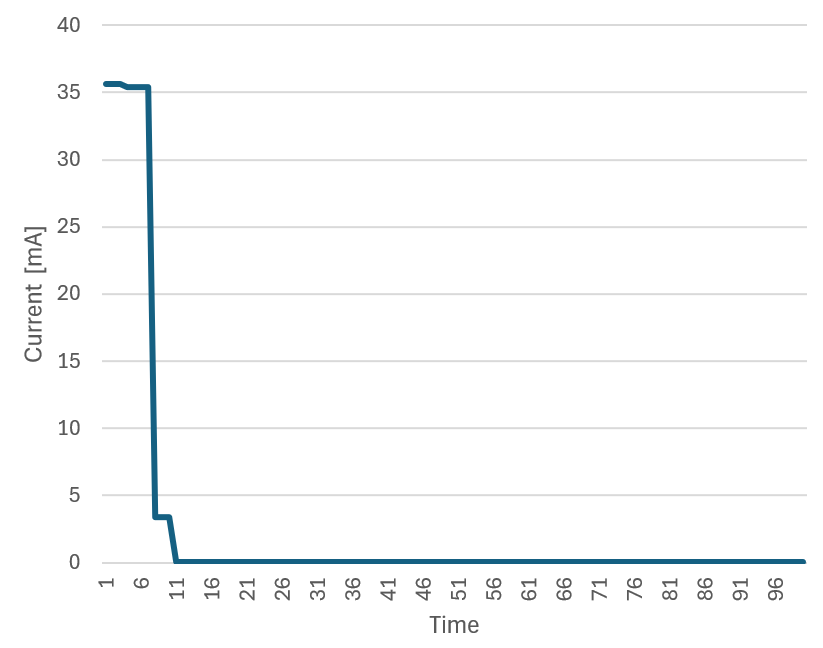
\includegraphics[width=0.55\textwidth]{figures/2_HW_figures/Standard_Cycle_Current_DC.png}
	\caption{Estimated DC/DC output current profile during the standard use cycle.}
	\label{fig:dcdc_current_cycle}
\end{figure}

The resulting loss estimation is reported in Table~\ref{tab:dcdc_loss_estimation}. 
The output power values are already averaged over the full standard use cycle. 
Therefore, for each region, the conversion loss is computed as:
\begin{equation}
	\label{eq:on_state_dcdc_region_loss}
	P_{loss,i} = P_{out,avg,i} \cdot \left(\frac{1}{\eta_i} - 1\right)
\end{equation}

\begin{table}[H]
	\centering
	\small
	\caption{DC/DC conversion loss estimation over the standard use cycle.}
	\label{tab:dcdc_loss_estimation}
	\begin{tabular}{@{}l c c c c c c@{}}
		\toprule
		\textbf{Region} & \textbf{\(I_{ref}\)} & \textbf{\(\eta\)} & \textbf{Time} & \textbf{\(I_{avg}\)} & \textbf{\(P_{out,avg}\)} & \textbf{\(P_{loss}\)} \\
		\midrule
		Low current &
		\(0.1\,\mathrm{mA}\) &
		\(70\%\) &
		\(90\%\) &
		\(0.01\,\mathrm{mA}\) &
		\(0.03\,\mathrm{mW}\) &
		\(0.01\,\mathrm{mW}\) \\
		
		Medium current &
		\(1\,\mathrm{mA}\) &
		\(80\%\) &
		\(10\%\) &
		\(2.59\,\mathrm{mA}\) &
		\(8.54\,\mathrm{mW}\) &
		\(2.13\,\mathrm{mW}\) \\
		
		High current &
		\(100\,\mathrm{mA}\) &
		\(85\%\) &
		\(0\%\) &
		\(0.00\,\mathrm{mA}\) &
		\(0.00\,\mathrm{mW}\) &
		\(0.00\,\mathrm{mW}\) \\
		\midrule
		Total &
		-- &
		-- &
		\(100\%\) &
		-- &
		-- &
		\(2.15\,\mathrm{mW}\) \\
		\bottomrule
	\end{tabular}
\end{table}

The total ON-state conversion loss is therefore:
\begin{equation}
	\label{eq:on_state_p_loss}
	P_{loss,ON} = \sum_i P_{loss,i} = 2.15\,\mathrm{mW}
\end{equation}

The quiescent power is evaluated under the worst-case input voltage, using the converter quiescent current reported in the datasheet~\cite{max77597_datasheet}:
\begin{equation}
	\label{eq:on_state_p_quiescent}
	P_{quiescent,ON} = V_{worst} \cdot I_{quiescent}
	= 21\,\mathrm{V} \cdot 1.1\,\mu\mathrm{A}
	\simeq 0.02\,\mathrm{mW}
\end{equation}

Using the DC/DC model defined in Section~\ref{sec:dcdc_loss_estimation}, the total DC/DC contribution during ON-state operation is:
\begin{equation}
	\label{eq:on_state_p_dcdc}
	P_{DC/DC,ON} = P_{quiescent,ON} + P_{loss,ON}
	= 0.02\,\mathrm{mW} + 2.15\,\mathrm{mW}
	= 2.17\,\mathrm{mW}
\end{equation}

The total power associated with the internal electronics is then:
\begin{equation}
	\label{eq:on_state_p_electronics}
	P_{electronics,ON} = P_{components,ON} + P_{DC/DC,ON}
	= 8.42\,\mathrm{mW} + 2.17\,\mathrm{mW}
	= 10.59\,\mathrm{mW}
\end{equation}


\paragraph{Power Distribution}
\label{sec:power_distribution}

Figure~\ref{fig:component_power_distribution} shows the relative contribution of the active electronics during the standard use cycle. 
The shunt power dissipation is not included in this chart, because it is much larger than the other contributions and would make the remaining component-level distribution unreadable.

\begin{figure}[H]
	\centering
	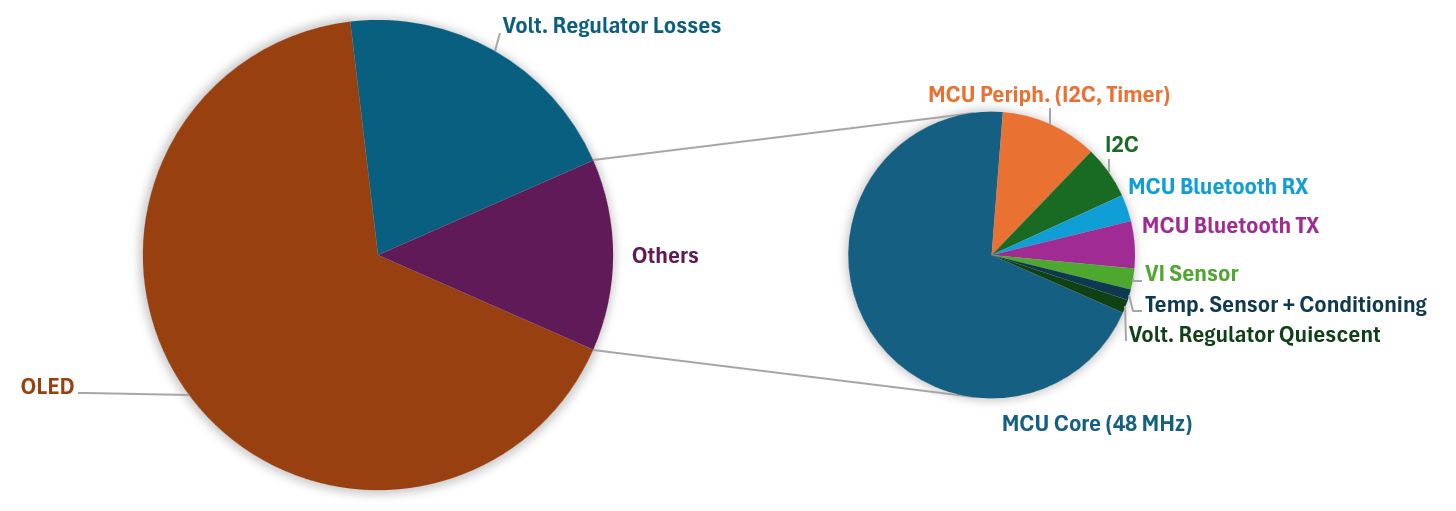
\includegraphics[width=0.95\textwidth]{figures/2_HW_figures/ON-state_Power_Distribution.png}
	\caption{Power distribution of the active electronics during the standard use cycle. The shunt dissipation is not included.}
	\label{fig:component_power_distribution}
\end{figure}

\paragraph{Shunt Power Dissipation}
\label{sec:shunt_power_dissipation}

The shunt resistor is placed in the measured USB power path. 
Its dissipation is therefore not related to the internal electronics duty cycle, but only to the current flowing through the monitored bus. 
Using the worst-case operating current, the shunt power is:
\begin{equation}
	\label{eq:on_state_p_shunt}
	P_{shunt,ON} = I_{worst}^{2} \cdot R_{shunt}
	= \left(5\,\mathrm{A}\right)^2 \cdot 0.01\,\Omega
	= 250\,\mathrm{mW}
\end{equation}


\subsubsection{Total ON-State Power Consumption and Efficiency}
\label{sec:total_on_state_power_consumption}

The total power dissipated by WattMate during ON-state operation is obtained by summing the shunt dissipation and the power required by the internal electronics. 
Using the internal electronics contribution computed in Equation~\ref{eq:on_state_p_electronics}:
\begin{equation}
	\label{eq:on_state_p_wattmate}
	P_{WattMate,ON} = P_{shunt,ON} + P_{electronics,ON}
	= 250\,\mathrm{mW} + 10.59\,\mathrm{mW}
	= 260.59\,\mathrm{mW}
\end{equation}

Under the worst-case operating condition of \(21\,\mathrm{V}\) and \(5\,\mathrm{A}\), the monitored bus power is:
\begin{equation}
	\label{eq:on_state_p_bus_worst}
	P_{bus,worst} = V_{worst} \cdot I_{worst}
	= 21\,\mathrm{V} \cdot 5\,\mathrm{A}
	= 105\,\mathrm{W}
\end{equation}

The corresponding ON-state efficiency is:
\begin{equation}
	\label{eq:on_state_efficiency}
	\eta_{ON}
	= \frac{P_{bus,worst}}{P_{bus,worst} + P_{WattMate,ON}}
	= \frac{105\,\mathrm{W}}{105\,\mathrm{W} + 0.26059\,\mathrm{W}}
	= 99.75\%
\end{equation}

This result satisfies the ON-state efficiency requirement, since the estimated efficiency is greater than \(99\%\) under the considered worst operating condition.



\subsection{Idle Consumption}
\label{sec:idle_consumption}

The idle consumption is evaluated using the same methodology introduced in Section~\ref{sec:power_estimation_methodology} and the same ON and idle current values defined in Section~\ref{sec:on_idle_currents_subsystems}. 
Only the duty cycles are changed, because the idle condition represents a different usage scenario.

In idle state, WattMate is powered and remains discoverable through BLE advertising, but no relevant power is assumed to flow through the monitored USB bus. 
Therefore, the shunt dissipation is considered null:
\begin{equation}
	\label{eq:idle_p_shunt}
	P_{shunt,idle} = 0
\end{equation}

The PAC1951 is kept in its idle sampling profile, while the I\textsuperscript{2}C bus, NTC branch, OLED display, and measurement-related peripherals are considered inactive. 
The only periodic active contribution is the BLE advertising transmission.

\paragraph{BLE advertising duty cycle.}
In idle state, WattMate remains discoverable through BLE advertising. 
The firmware uses a temporary fast advertising interval after startup or user interaction, but the steady idle condition is represented by the slow advertising interval:
\begin{equation}
	T_{adv,idle} = 1000\,\mathrm{ms}
\end{equation}

The idle advertising configuration is summarized in Table~\ref{tab:idle_ble_advertising_config}. 
Only the periodic advertising packets are included in the baseline idle estimate. 
Scan responses are not periodic and are transmitted only when an external scanner sends a scan request, so they are not included in the quiet-idle power calculation.

\begin{table}[H]
	\centering
	\small
	\caption{BLE advertising configuration used for the idle power estimate.}
	\label{tab:idle_ble_advertising_config}
	\begin{tabular}{@{}l l@{}}
		\toprule
		\textbf{Parameter} & \textbf{Idle advertising configuration} \\
		\midrule
		Advertising interval & \(1000\,\mathrm{ms}\) \\
		Advertising type & Legacy, connectable, scannable \\
		Advertising channels & Primary channels 37, 38, and 39 \\
		Advertising data length & \(13\,\mathrm{B}\) \\
		Advertising data content & BLE flags and complete local name \texttt{WattMate} \\
		\bottomrule
	\end{tabular}
\end{table}

The advertising packet airtime is estimated using the same simplified packet-level model adopted for the connected BLE radio estimate. 
For a legacy advertising packet, the on-air data include the preamble, access address, advertising header, advertiser address, advertising payload, and CRC:
\begin{equation}
	N_{adv} = 1\,\mathrm{B} + 4\,\mathrm{B} + 2\,\mathrm{B} + 6\,\mathrm{B} + 13\,\mathrm{B} + 3\,\mathrm{B}
	= 29\,\mathrm{B}
\end{equation}

Using the LE \(1\,\mathrm{Mbit/s}\) PHY, the airtime of one advertising packet is:
\begin{equation}
	t_{adv} = 8 \cdot N_{adv} \cdot 1\,\mu\mathrm{s}
	= 8 \cdot 29\,\mu\mathrm{s}
	= 232\,\mu\mathrm{s}
\end{equation}

Since one advertising event transmits the packet on the three primary advertising channels, the TX airtime of one idle advertising event is:
\begin{equation}
	t_{adv,event} = 3 \cdot t_{adv}
	= 3 \cdot 232\,\mu\mathrm{s}
	= 696\,\mu\mathrm{s}
\end{equation}

The resulting BLE advertising TX duty cycle is therefore:
\begin{equation}
	\label{eq:idle_ble_adv_duty}
	D_{BLE,TX,adv} = \frac{t_{adv,event}}{T_{adv,idle}}
	= \frac{696\,\mu\mathrm{s}}{1000\,\mathrm{ms}}
	= 0.0696\%
\end{equation}

The firmware uses the default \(0\,\mathrm{dBm}\) advertising TX power. 
The \(+5\,\mathrm{dBm}\) TX current reported in Table~\ref{tab:on_idle_currents_subsystems} is therefore a conservative upper-bound value for the idle estimate.


\paragraph{Idle duty-cycle summary.}
After defining the BLE advertising TX duty cycle, the complete set of idle duty-cycle assumptions can be summarized. 
A duty cycle equal to zero means that the corresponding subsystem is not actively used during idle operation and its idle current, defined in Table~\ref{tab:on_idle_currents_subsystems}, is applied.

The MCU core and the auxiliary MCU peripherals are assigned a conservative \(1\%\) active duty cycle. 
This margin accounts for the periodic wake-up activity required to manage BLE advertising and is selected with the same conservative approach discussed for the ON-state estimate in Paragraph~\ref{par:on_state_mcu_core_peripherals}.

\begin{table}[H]
	\centering
	\small
	\setlength{\tabcolsep}{7pt}
	\renewcommand{\arraystretch}{1.08}
	\caption{Idle-state duty-cycle assumptions.}
	\label{tab:idle_duty_cycle_summary}
	\begin{tabularx}{\textwidth}{@{}l c X@{}}
		\toprule
		\textbf{Subsystem} & \textbf{Duty cycle} & \textbf{Idle-state assumption} \\
		\midrule
		MCU core &
		\(1\%\) &
		Conservative margin for BLE advertising wake-up activity. \\
		
		I\textsuperscript{2}C block &
		\(0\%\) &
		No periodic I\textsuperscript{2}C traffic in idle. \\
		
		Other MCU peripherals &
		\(1\%\) &
		Conservative margin for timer and BLE/RF control activity. \\
		
		PAC1951 sensor &
		\(0\%\) &
		Idle sampling profile, so the idle current is applied. \\
		
		NTC branch &
		\(0\%\) &
		Temperature sensing branch disabled. \\
		
		OLED display &
		\(0\%\) &
		Display disabled. \\
		
		BLE TX &
		\(0.0696\%\) &
		Periodic legacy advertising transmission, from Equation~\ref{eq:idle_ble_adv_duty}. \\
		
		BLE RX &
		\(0\%\) &
		No connected-link RX activity in quiet idle. \\
		\bottomrule
	\end{tabularx}
\end{table}



\paragraph{Average Idle-State Component Consumption}
\label{sec:idle_component_consumption}

Table~\ref{tab:idle_component_consumption} summarizes the average current and power contribution of the subsystems that consume power during idle operation. 
The average current is computed using Equation~\ref{current_avg_formula}, while the average power is obtained from the regulated internal supply voltage \(V_{DD}=3.3\,\mathrm{V}\).

\begin{table}[H]
	\centering
	\small
	\setlength{\tabcolsep}{9pt}
	\caption{Average current and power contribution during idle operation.}
	\label{tab:idle_component_consumption}
	\begin{tabular}{@{}l r r c r r@{}}
		\toprule
		\textbf{Component} & \textbf{\(I_{ON}\)} & \textbf{\(I_{idle}\)} & \textbf{\(D\)} & \textbf{\(I_{avg}\)} & \textbf{\(P_{avg}\)} \\
		\midrule
		MCU core &
		\(2.94\,\mathrm{mA}\) &
		\(0.0011\,\mathrm{mA}\) &
		\(1\%\) &
		\(0.030\,\mathrm{mA}\) &
		\(0.10\,\mathrm{mW}\) \\
		
		Other MCU peripherals &
		\(0.463\,\mathrm{mA}\) &
		\(0\,\mathrm{mA}\) &
		\(1\%\) &
		\(0.005\,\mathrm{mA}\) &
		\(0.02\,\mathrm{mW}\) \\
		
		PAC1951 sensor &
		\(0.010\,\mathrm{mA}\) &
		\(0.005\,\mathrm{mA}\) &
		\(0\%\) &
		\(0.005\,\mathrm{mA}\) &
		\(0.02\,\mathrm{mW}\) \\
		
		BLE TX &
		\(9.10\,\mathrm{mA}\) &
		\(0\,\mathrm{mA}\) &
		\(0.0696\%\) &
		\(0.006\,\mathrm{mA}\) &
		\(0.02\,\mathrm{mW}\) \\
		\midrule
		Total &
		-- &
		-- &
		-- &
		\(0.046\,\mathrm{mA}\) &
		\(0.15\,\mathrm{mW}\) \\
		\bottomrule
	\end{tabular}
\end{table}


\subsubsection{Idle DC/DC Converter Loss Estimation}
\label{sec:idle_dcdc_loss_estimation}

The idle DC/DC loss is evaluated using the same procedure adopted for the ON-state case in Section~\ref{sec:on_state_dcdc_loss_estimation}. 
In idle operation, the load current remains very low for most of the time, but a small fraction of the cycle is still associated with a higher current level due to the periodic BLE advertising activity. 
For this reason, the idle current profile is divided into the same representative current regions used for the ON-state estimate.

The resulting loss estimation is reported in Table~\ref{tab:idle_dcdc_loss_estimation}. 
As in the ON-state case, the output power values are already averaged over the full idle cycle, and the conversion loss is computed from the efficiency of each current region.

\begin{table}[H]
	\centering
	\small
	\caption{DC/DC conversion loss estimation during idle operation.}
	\label{tab:idle_dcdc_loss_estimation}
	\begin{tabular}{@{}l c c c c c c@{}}
		\toprule
		\textbf{Region} & \textbf{\(I_{ref}\)} & \textbf{\(\eta\)} & \textbf{Time} & \textbf{\(I_{avg}\)} & \textbf{\(P_{out,avg}\)} & \textbf{\(P_{loss}\)} \\
		\midrule
		Low current &
		\(0.01\,\mathrm{mA}\) &
		\(40\%\) &
		\(99\%\) &
		\(0.01\,\mathrm{mA}\) &
		\(0.02\,\mathrm{mW}\) &
		\(0.03\,\mathrm{mW}\) \\
		
		Medium current &
		\(1\,\mathrm{mA}\) &
		\(80\%\) &
		\(1\%\) &
		\(0.03\,\mathrm{mA}\) &
		\(0.11\,\mathrm{mW}\) &
		\(0.03\,\mathrm{mW}\) \\
		
		High current &
		\(100\,\mathrm{mA}\) &
		\(85\%\) &
		\(0\%\) &
		\(0.00\,\mathrm{mA}\) &
		\(0.00\,\mathrm{mW}\) &
		\(0.00\,\mathrm{mW}\) \\
		\midrule
		Total &
		-- &
		-- &
		\(100\%\) &
		-- &
		-- &
		\(0.06\,\mathrm{mW}\) \\
		\bottomrule
	\end{tabular}
\end{table}

The quiescent power is evaluated using the same worst-case input voltage defined for the ON-state efficiency evaluation:
\begin{equation}
	\label{eq:idle_p_quiescent}
	P_{quiescent,idle} = V_{worst} \cdot I_{quiescent}
	= 21\,\mathrm{V} \cdot 1.1\,\mu\mathrm{A}
	\simeq 0.02\,\mathrm{mW}
\end{equation}

Using the DC/DC model defined in Section~\ref{sec:dcdc_loss_estimation}, the total DC/DC contribution during idle operation is:
\begin{equation}
	\label{eq:idle_p_dcdc}
	P_{DC/DC,idle} = P_{loss,idle} + P_{quiescent,idle}
	= 0.06\,\mathrm{mW} + 0.02\,\mathrm{mW}
	= 0.08\,\mathrm{mW}
\end{equation}

The total power associated with the internal electronics during idle operation is then:
\begin{equation}
	\label{eq:idle_p_electronics}
	P_{electronics,idle} = P_{components,idle} + P_{DC/DC,idle}
	= 0.15\,\mathrm{mW} + 0.08\,\mathrm{mW}
	= 0.23\,\mathrm{mW}
\end{equation}

\subsubsection{Total Idle-State Power Consumption}
\label{sec:total_idle_state_power_consumption}

In idle state, WattMate is powered, but no relevant current is assumed to flow through the monitored USB power bus. 
Since the idle shunt dissipation has already been defined as zero in Equation~\ref{eq:idle_p_shunt}, the total idle-state power consumption is only given by the internal electronics contribution:
\begin{equation}
	\label{eq:idle_p_wattmate}
	P_{WattMate,idle} = P_{electronics,idle} + P_{shunt,idle}
	= 0.23\,\mathrm{mW} + 0\,\mathrm{mW}
	= 0.23\,\mathrm{mW}
\end{equation}

Figure~\ref{fig:idle_power_distribution} reports the distribution of the idle-state power consumption. 
As for the ON-state distribution in Figure~\ref{fig:component_power_distribution}, the chart separates the main contributors and highlights the smaller contributions in a secondary pie chart.

\begin{figure}[H]
	\centering
	\includegraphics[width=0.95\textwidth]{figures/2_HW_figures/IDLE-State_Power_Distribution.png}
	\caption{Power distribution of WattMate during idle-state operation.}
	\label{fig:idle_power_distribution}
\end{figure}


\paragraph{Idle battery endurance.}
Considering a battery energy of \(32\,\mathrm{Wh}\), the ideal idle endurance is estimated as:
\begin{equation}
	\label{eq:idle_endurance_hours}
	t_{idle} = \frac{E_{battery}}{P_{WattMate,idle}}
	= \frac{32\,\mathrm{Wh}}{0.00023\,\mathrm{W}}
	\simeq 1.39 \cdot 10^{5}\,\mathrm{h}
\end{equation}

which corresponds to:
\begin{equation}
	\label{eq:idle_endurance_days}
	t_{idle,days} = \frac{t_{idle}}{24}
	= \frac{1.39 \cdot 10^{5}}{24}
	\simeq 5.80 \cdot 10^{3}\,\mathrm{days}
\end{equation}

This value represents an ideal electronics-only endurance. 
In a real product, the effective long-term idle lifetime would also be limited by battery self-discharge and by leakage currents not included in this design-stage estimate.